\documentclass{beamer}
\usetheme{metropolis}
\usepackage{graphicx}
\usepackage[utf8]{inputenc}
\usepackage[russian]{babel}

\begin{document}

% Конфигурация титульного листа
%---------------------------
\title{Разработка итерационных алгоритмов поиска автоморфизмов
и изоморфизмов комбинаторных объектов.}

\institute{Московский государственный университет имени М.В.Ломоносова\\
Факультет вычислительной математики и кибернетики\\
Кафедра информационной безопасности}

\author{\textit{\underline{Автор:}}\\ Ефремов Степан Сергеевич (419 группа)\\ \\
\textit{\underline {Научный руководитель:}}\\ доцент, к.ф.- м.н.\\ Егоров Владимир Николаевич}

\date{}

%---------------------------


% 1 слайд - титульная страница
%---------------------------
\begin{frame}{}
\titlepage
\end{frame}
%---------------------------


% 2 слайд - содержание
%---------------------------
\begin{frame}{Содержание}
\tableofcontents
\end{frame} 
%---------------------------


\section{Постановка задачи}
% 3 слайд
%---------------------------
\begin{frame}{Постановка задачи}
\small
\begin{enumerate}
\item Исследование свойств алгоритма:
\begin{itemize}
\scriptsize
\item Определение класса решаемых задач
\item Вероятностная сложность
\item Теоретическая возможность распараллеливания
\end{itemize}
\item Задачи, связанные с реализацией для ПК:
\begin{itemize}
\scriptsize
\item Реализация в виде программы с графическим интерфейсом
\item Эксперименты поиска автоморфизмов на известных графах
\item Поддержа функционала нахождения изоморфного вложения графов
\end{itemize}
\item Задачи, связанные с реализацией для суперкомьютера:
\begin{itemize}
\scriptsize
\item Модернизация алгоритма на основе исследований
\item Реализация в виде программы для запуска на суперкомпьютере
\item Эксперименты поиска автоморфизмов графов на суперкомпьютере
\end{itemize}
\item Исследование практического применения алгоритма для задачи Коши
\end{enumerate}
\end{frame} 
%---------------------------


\section{Существующие решения}
% 5 слайд
%---------------------------
\begin{frame}{Направления исследований}
На данный момент сформированы два направления изучения и решения проблемы поиска изоморфизмов графов:
\begin{itemize}
\item Теоретическое, в котором проблема изоморфизма рассматривается с позиций современной теории сложности алгоритмов и вычислений (подход использует понятие инвариантов графа).

\item Практическое, предполагающее разработку алгоритмов, решающих задачу изоморфизма графов за <<практически приемлемое>> время (направленный перебор).
\end{itemize}
\end{frame}
%---------------------------


% 6 слайд
%---------------------------
\begin{frame}{Сравнение сложностей алгоритмов}

\begin{table}[h]
\centering
\small
\begin{tabular}[t]{|l|l|l|}
\hline
\textbf{Алгоритм} & \textbf{Ограничения} & \textbf{Сложность}\\
\hline
Полный перебор & без ограничений & $n!$\\
\hline
Егоров В.Н., Егоров А.В. & без ограничений & $O(n^2(\frac{e}{2})^{\ln(n)^2} \ln(n))$\\
\hline
László Babai, Eugene M. & без ограничений & $O(e^{-n^{\frac{1}{2} + c}})$\\
\hline
László Babai & cильно регулярные & $O(e^(2fi \log2 n)$\\
\hline
Vaibhav Amit Patel & специальный вид & $O(n^4)$\\
\hline
\end{tabular}
\caption{Алгоритмы поиска автоморфизмов}
\end{table}

\end{frame}
%---------------------------


\section{Разработанные решения}

%---------------------------
\begin{frame}{Модернизированный алгоритм}

Разработан алгоритм с вероятностной сложностью:

$$O(n^2(\frac{e}{2})^{\ln(n)^2} \ln(n))$$

Алгоритм является универсальным и может применяться для решения большого количества задач (как минимум всех указанных в пункте 4.1 дипломной работы).

Написанная программа с интерфейсом имеет масштабируемые функционал. На данный момент поддерживает функционал решения следующих задач:

\begin{itemize}
\item Поиск автоморфизмов
\item Поиск изоморфизмов
\item Поиск гомоморфизмов
\item Решение задачи Коша в подстановках
\end{itemize}

\end{frame}
%---------------------------


%---------------------------
\begin{frame}{Разработанные приложения}

Разработано 2 программы:

\begin{enumerate}
\item Приложение с графическим интерфейсом, написанное на $Qt$
\begin{itemize}
\item не поддерживает распараллеливание
\item справляется с графами размера до 500 вершин
\item удобный анализ графов
\item помимо нахождения автоморфизмов, решает задачи изоморфизма и гомоморфизма графов
\end{itemize} 
\item Программа на языки $C++$ с поддержкой $OpenMPI$
\begin{itemize}
\item поддерживает распараллеливание средствами $OpenMPI$
\item помимо нахождения автоморфизмов, сохраняет много информации для анализа графов с большим количеством вершин
\end{itemize} 
\end{enumerate} 

\end{frame}
%---------------------------

% 7 слайд
%---------------------------
\begin{frame}{Тестирование на суперкомпьютере}

Набор и границы значений изменяемых параметров запуска реализации алгоритма: 

\begin{enumerate}
\item Число процессоров [4 : 128] с шагом $ 2^n$ (точки отображены с шагом 4, усреднив результаты);
\item Размер матрицы [300 : 1000].
\end{enumerate}

\end{frame}
%---------------------------




\section{Результаты} 

% 8 слайд
%---------------------------
\begin{frame}{Изменение производительности}

\begin{figure}[ht]
\centering 
    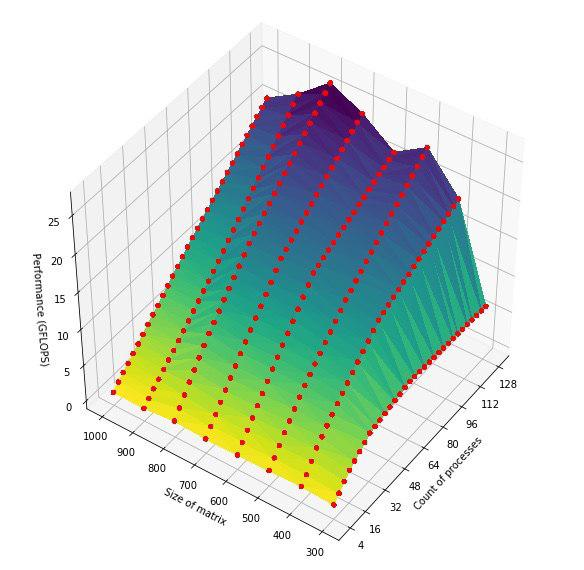
\includegraphics[scale=0.4]{../image/p.jpg}
\end{figure}

\end{frame}
%---------------------------



% слайд
%---------------------------
\begin{frame}{Изменение эффективности}

\begin{figure}[ht]
\centering 
    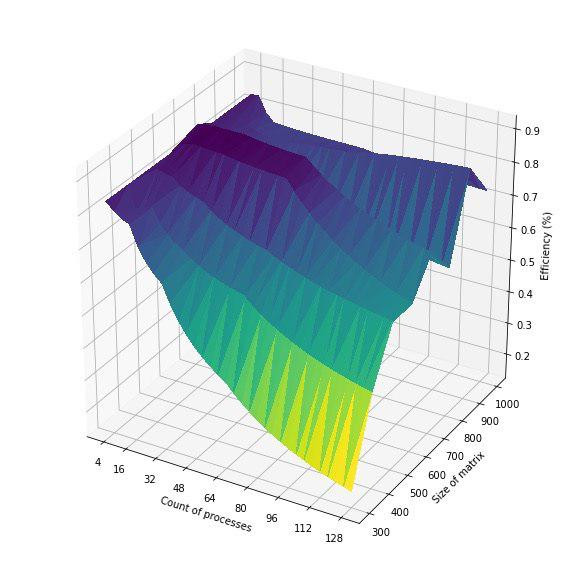
\includegraphics[scale=0.4]{../image/ef.jpg}
\end{figure}

\end{frame}
%---------------------------


\section{Положения, выносимые на защиту}
% 11 слайд
%---------------------------
\begin{frame}{Положения, выносимые на защиту}

Разработка итерационного алгоритма поиска автоморфизмов графов:
\begin{itemize}
\item Выполнена модернизация алгоритма
\item Сформулировано утверждение вероятностной сложности алгоритма
\item Реализовано 2 програмы: с графическим интерфейсом для удобного использования, с консольным интерфейсом для запуска на суперкомпьютере\item Проведены опыты на суперкомпьютере <<Ломоносов>>
\end{itemize}

\end{frame}
%---------------------------


\end{document}